\documentclass[fleqn,10pt]{wlscirep}

\usepackage[utf8]{inputenc}
\usepackage[T1]{fontenc}
\usepackage{bm}
\usepackage{siunitx}
\usepackage{amsmath}
\usepackage{nccmath}
\usepackage{indentfirst}
\usepackage{multirow}
\usepackage[version=3]{mhchem}


\DeclareSIUnit{\Bit}{~Bit}
\title{Improving Pooling-Strategies for Increasing the Test Capacity and Reliability of RT-qPCR of Samples out of Populations with low Prevalence} 


%improve order of authors maybe use a circle (it's a really old list.)
\author[*]{Kuo-Yi Chao}
\author[*]{Leonhard Kuboschek}
\author[*]{Leo T. Peters}
\author[*]{Christoph Schierholt}
\author[*]{Pranav Kumar Shadamarshan}

%\affil[1]{Affiliation, Department, City, Country}
%\affil[2]{Affiliation, Department, City, Country}

\affil[*]{All authors are equal in this report, the names are sorted alphabetically by last name}


\begin{abstract}

SARS-COV-2 has spread through the world and wreaked havoc to unforeseen levels. The lack of information about the virus has specifically made it difficult, while in the pursuit it has baffled medical experts due to the lack of readily available testing kits. RT-qPCR stands as the golden standard procedure for diagnosis of COVID-19. Here, we propose a strategy to increase the testing capability by pooling multiple samples. It is a pure strategic manipulation by mixing samples with the aim of obtaining maximum possible information, without excess uses of resources.


\end{abstract}
\begin{document}

\flushbottom
\maketitle

\thispagestyle{empty}

\section{Introduction}

SARS-COV-2 (Severe acute respiratory syndrome coronavirus 2) or 2019-nCOV is a type of bat-borne virus that causes respiratory illness. It is the mutational successor to SARS-COV-1 which was identified in the 2003 outbreak largely in Asia. They are a class of RNA viruses that causes coronavirus disease 2019 (covid-19). With no immunity in the community and asymptomatic transmissions, covid-19 has been announced a pandemic and a matter of public health emergency. Covid-19 has been taking over the world like a wildfire and the economies of countries have succumbed to it. The main reason for this letdown is unavailability of ample testing kits due to inefficient testing.\\

With faster and efficient testing strategy, a country knows where it stands amidst this pandemic. For instance, South Korea in the first week of its critical period had already conducted 300,000 tests, establishing 600 test centres across the country. It had halved the number of infections in just a week [1]. On the other end of the spectrum, Italy and the US has/is failing to cope up with the pandemic. So much so that Italy could not keep up with the pandemic because they did not know where they stood in the curve because of the inefficiency in testing samples. Efficient testing could give more information on the current situation in the pandemic and allow governments to take more appropriate measures. At a large scale, it could reward the community by flattening the curve faster and decreasing the R0. Randomized community testing could also be made possible which is highly advantageous to isolate asymptomatic infected people disrupting the infection chain. The delay in testing has and is still costing lives [1-3]. The take home message from these scenarios is that high capacity testing provides more information upon which a country could take a standpoint and act in preparedness. We require a method to increase the efficiency of testing without excess resources, or labour. So, we propose a strategy for efficient testing of SARS-COV-2 by sample pooling.


\section{Methods}

\subsection{Information Theory}
A measure for the amount of information is the so called \glqq entropy\grqq{} and is associated with the unit \si{\Bit}. It forms the basis of information theory, which was initially developed by Shannon \cite{Shannon} and is mainly used in communication engineering. In this paper we will apply it to pool testing in order to estimate the potential of an optimal pooling strategy and to compare the developed strategies to such optimal performance.\\

The relevance of information theory in the context of large scale testing can be understood as follows: The total amount of information on the patients state of a population is bounded, as we are looking at a finite number of people with a binary state (infected or not infected). By applying pool testing, the information obtained by a test can be increased, which allows us to require less tests in order to evaluate the peoples state.\\

The amount of information carried by a Bernoulli distributed (or binary) random variable can be closely related to the information carried by a diagnostical test, which also yields a binary result (positive or negative).\\

Information theory tells us, that the entropy of such random variable is maximized, if its both outcomes are equally distributed. In this case the amount of information is \SI{1}{\Bit}. This is also the maximum information obtained by a single diagnostic test that does not allow any errors in result.\\

In the case of single testing with ideal tests the amount of information obtained by one test is equal to the amount of information carried by one patients state. This is why we need exactly one test per person if we conduct single testing. The entropy of the populations state depends on the prevalence and can be estimated by regarding each patient as a binary random variable with probability equalling to the prevalence $p_{inf}$:\\

\begin{ceqn}
\begin{equation}
H(p_{inf}) = -p_{inf} \cdot \log_2(p_{inf})-(1-p_{inf}) \cdot \log_2(p_{inf}) \si{\Bit}
\end{equation}
\end{ceqn}

\begin{figure}[ht]
	\centering
	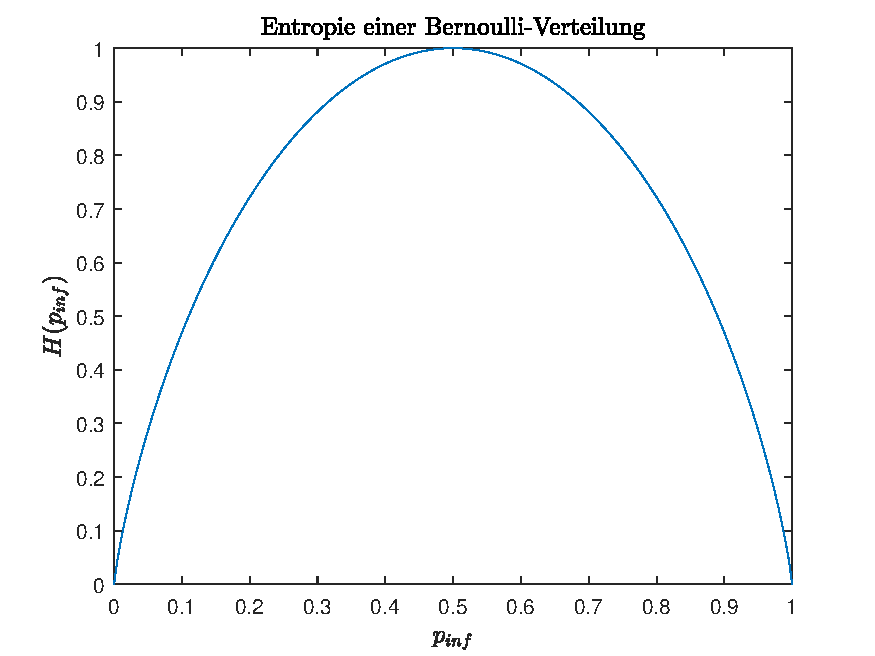
\includegraphics[]{pics/Bin_Entropie.pdf}
	\caption{Amount of Information obtained by a single and ideal test vs. prevalence $p_{inf}$}
	\label{fig:bin_entropie}
\end{figure}

Fig. \ref{fig:bin_entropie} shows a maximum in entropy of a test, if its outcome is equally distributed. It is interesting to note, that the entropy only varies slightly for small deviations from the optimum, while it drops to zero, when the prevalence is $0$. This means that single testing cannot be used efficiently at low prevalences. Prevalences above $0.5$ will not be regarded in this work.\\

This means that single testing cannot be used efficiently at low prevalences. Prevalences above 0.5 will not be regarded in this work. By pooling samples together, we end up with a mix. We can increase the probability of such a mix containing at least one positive sample by adding more samples. For low prevalence this leads to a higher amount of information obtained by one test performed on this mix, when comparing it to single testing.
This will be further carried out in section \ref{sec:analytics}.\\



Another important measure from information theory is mutual information. It indicates how much information of one random distribution can be obtained by another random distribution. If a diagnostic test was never leading to an error, the distribution of a persons state and of the test result a closely coupled, which results in the mutual information being equal to the entropy of the person's state. If however errors occur, the information lost during the conduction of a test (through false negatives and false positives) is the difference between the information of the person's state and the mutual information, which is depicted in fig. \ref{fig:mutual_information}. In the case of an imperfect diagnostic test, it can be useful to maximize the mutual information between the population's state and the test results instead of maximizing the entropy.\\

\begin{figure}[ht]
	\centering
	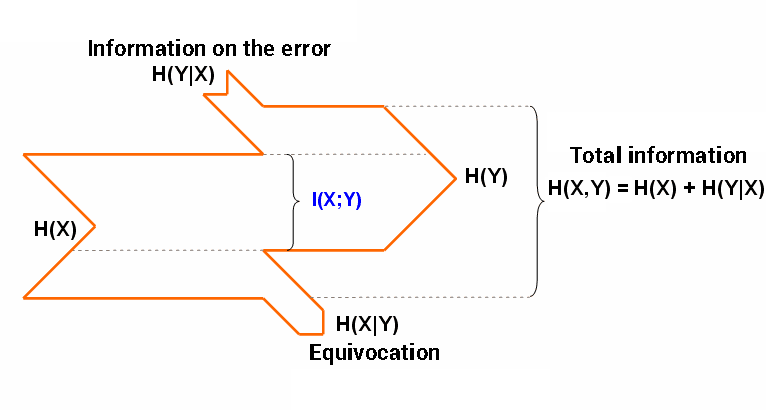
\includegraphics[width=0.7\linewidth]{pics/Entroy_XY_Eng.png}
	\caption{Mutual information of two sources where X is the Sender and Y is the receiver. }
	\label{fig:mutual_information}
\end{figure}

Another use for the mutual information is the evaluation of conducting multiple diagnostic tests on subsets of a bigger pool of samples. Just as it is desirable to increase the mutual information between the population's state and the test results, it is also desirable to decrease the mutual information between the test results of multiple tests. This originates in the idea, that obtaining the same information by multiple tests will not increase the overall information retrieved. The concept of mutual information will only be used as an instrument to emphasize differences between strategies, while it will not be used for optimization as part of this work.


\subsection{RT-qPCR}
Detection of the viral infection in patient samples is performed by Reverse transcription- quantitative polymerase chain reaction (RT-qPCR) analysis. It works by selectively amplifying the viral RNA gene and by detecting the amplified viral gene. It is the most common analytical technique used to analyze SARS-COV-2 in the current pandemic situation. RT-qPCR could be done in a single step or a longer double step method. WHO recommends either of these types. From publications surfacing around the world, the common trend is a one-step RT-qPCR.\\

The analytical technique only works on DNA. So, it is imperative to convert the viral RNA to DNA in order to be detected. The first protocol is to convert the existing RNA to DNA (Reverse Transcription). Followed by the amplification and detection of the DNA samples (quantitative PCR). The amplification and detection takes place in several cycles of the analysis. Each cycle takes \SI{45}{seconds}. 45 such cycles are performed and a readout is taken at the end of each cycle. Under the presence of the viral gene the readout value increases with every cycle and surpassess the threshold (above noise levels), but under the absence of any infection the readout stays below the threshold in all cycles. For the sake of error corrections, any readout that surpassess the threshold in late cycles might be considered false positive.\\

WHO recommends a three assay workflow, first line screening, confirmatory and discriminatory assays. First line assay confirms the presence of E gene, which would confirm the presence of Bat related viruses in the sample. Confirmatory assay (RdRp assay I) proclaims the presence of SARS related viruses. Finally discriminatory assay (RdRp assay II) provides the verdict for the novel SARS-COV-2 infection in the sample. One assay succeeding the other only in the case of a positive result.\\

A typical commercial RT-qPCR reagent consists of a 2x reaction mixture, BSA (Bovine Serum Albumin) to increase efficiency, Primers for amplification of selective genes and probes for the detection of selective genes. The design of primers and probes play a major role in the RT-qPCR analysis. A probe is a small nucleotide stretch (TaqMan probe) that attaches to the said viral gene and fluoresces upon each amplification cycle. This fluorescence is the readout at the end of each cycle. The primer and probe designs have been optimized and reported by WHO as follows:
\begin{table}
\begin{center}
	\begin{tabular}{ |c|l|l| } 
		\hline
		Assay & oligonucleotide ID/ use & sequence 5’ $\rightarrow$ 3’ \\ 
		\hline
		 \multirow{3}{*}{E gene} & E Sarbeco F2 (Forward) & ACAGGTACGTTAATAGTTAATAGCGT \\  \cline{2-3}
		  & E Sarbeco R2 (Reverse) & ATATTGCAGCAGTACGCACACA \\ \cline{2-3}
		 & E Sarbeco P1 (probe for detection of E gene) & FAM-ACACTAGCCATCCTTACTGCGCTTCG-BBQ \\ \cline{2-3}
		\hline
		 \multirow{4}{*}{RdRp gene} & RdRP SARSr-F2 (Forward) & GTGARATGGTCATGTGTGGCGG \\  \cline{2-3}
		& RdRP SARSr-R1 (Reverse) & CARATGTTAAASACACTATTAGCATA \\ \cline{2-3}
		& RdRP SARSr-P2 (detects only SARS-COV-2) & FAM-CAGGTGGAACCTCATCAGGAGATGC-BBQ \\ \cline{2-3}
		& RdRP SARSr-P1 (detects all bat related SARS-CoVs) & FAM-CCAGGTGGWACRTCATCMGGTGATGC-BBQ \\
		\cline{1-3}
		


	\end{tabular}
  	\caption{Primers and Probes}
	\label{tab:primes}
\end{center}
\end{table}

The reaction mixture has \SI{25}{\micro\litre} - \SI{5}{\micro\litre} of RNA, \SI{12.5}{\micro\litre} of 2x reaction buffer (made for one-step RT-qPCR with Platinum Taq Polymerase) \SI{1}{\micro\litre} of reverse transcriptase, \SI{0.4}{\micro\litre} of 50 mM \ce{MgSO4}, \SI{1}{\micro\litre} of required primers, \SI{0.5}{\micro\litre} of required probes and made up for the rest of the volume with sterile RNase free water to make \SI{25}{\micro\litre}. Thermal cycling is performed at 55°C for 10 min for reverse transcription, followed by 95°C for \SI{3}{\minute} and then 45 cycles of 95°C for \SI{15}{\second}, 58°C for \SI{30}{\second}.


\subsection{Assumptions}

In order to examine the effect of our pooling strategies, we implemented two models of the PCR (PCR simple and PCR dilution dependent) with varying degrees of realism. Another assumption addresses the distribution of viral loads within the patients.

\subsubsection{PCR simple}

PCR is a highly sensitive and specific technique. Hence, a tiny mishandling or variation would go a long way in the end result. The number of reagents added at very small amounts call for critical experimental handling. Other issues lie in the handling, transportation and storage of the clinical samples. With proper experienced manpower sensitivity is pointed to $98 \%$ and specificity at $99 \%$. The modelling in this case does not encompass the concentration, thermal cycles of qPCR run or other chemical parameters. Instead, the model considers whether any sample within a pool is positive. After applying the confusion matrix (based on the sensitivity and specificity), the output is generated accordingly. A limitation of this model is that it does not reflect the dilution of samples in pools, which will overrate the performance of sample pooling. On the other hand, the correlation of concentration between pools is not being considered, which will underrate its performance.


\subsubsection{PCR dilution dependent}
PCR is a quantitative technique and the results are highly affected by the initial viral gene content. The concentration of viral genes in a sample is denoted by copies/ml. A qPCR analysis requires a sample with a minimum content of viral copies/ml in order to detect it. This is known as the limit of detection (LOD). It is important to know the LOD of the E genes and the RdRp genes, as sample pooling will effectively lower the copies of the viral gene in the samples. The LOD for E gene is found to be 6.65 ± 2.95 copies/reaction and for RdRP 5.15 ± 2.45 copies/reaction.\\

For our model we use linear interpolation between 4 copies/reaction (\SI{0}{\percent}) and 10 copies/reaction (\SI{99.5}{\percent}) to determine the sensitivity. It remains at \SI{99}{\percent} for concentrations above 10 copies/ml as depicted in fig. \ref{LOD}. The specificity is not modelled concentration dependent and is set to \SI{99}{\percent}. 


\subsubsection{Viral Load}
The severity of the viral infection is characterized by its number of RNA copies in the patient sample. Clinical samples have shown around 1.6 x 106 RNA copies/ml [5]. The minimum amount required to analyse the sample is 400 RNA copies/ml [6].\\

This would technically mean that we could dilute a sample 4000 times and still be able to detect it. Pooling multiple samples would dilute the samples, but within a certain range would still be detectable. A test concluded that an interpretable signal was obtainable by pooling 32 samples together [7]. In our model we generate a discrete viral load distribution $c_{vir}$, which we chose by inspection. For effects introduced by the dilution we assume a binomial distribution of the resulting virus concentration, as we are dealing with discrete particles on such a low scale. \\

We assume that \SI{1}{\milli\liter} with $n_{vir} = c_{vir} \cdot \SI{1}{\milli\liter}$ RNA copies is being taken from each patient (where this number does not affect the outcome too much - it simply has to be chosen sufficiently big). From that volume $\frac{\SI{5}{\micro\liter}}{n_{pool}}$ where $n_{pool}$ denotes the number of samples per pool is being mixed. The model from the binomial distribution results from the thought, that each virus particle within that \SI{1}{\milli\liter} is equally distributed and therefore within the final mix with a probability $p_{in pool} = \frac{\SI{5}{\micro\liter}}{n_{pool} \cdot \SI{1}{\milli\liter}} = \frac{1}{200 \cdot n_{pool}}$. As $n_{vir} \geq 50$ and $p_{in pool} \leq 0.05$ it is safe to use the poisson-approximation \cite{poisson_approx}, which can be calculated faster in our simulation.



%let us insert the distribution of viral load as a histogram or table here.

\subsection{Strategy Evaluation Measure}
Common measures for evaluating the quality or correctness of a test are the sensitivity and the specificity.
\begin{itemize}
	\item Sensitivity is the probability that the test conducted on an infected person turns positive. $Sensitivity = \frac{TP}{TP+FN}$ The reasons for the sensitivity to be suboptimal in the case of RT-qPCR for SARS-CoV-2 can be
	\subitem low viral load of the patient
	\subitem poor extraction of the sample from the patient
	\subitem too little virus particles in the sample
	\subitem other handling errors
\end{itemize}

\subsection{Modelling Strategies}
- Monte Carlo Simulation in MATLAB 

- Indiv Testing (no MC needed)

- State of the Art Pool Testing

Our aim for the strategies is to pool multiple sample together for better data obtainment. For this we have several pooling-approaches in mind.
The first one we called CoSplit. This approach is the only approach we simulated yet. Aim of CoSplit is to get the maximum information gain out of the first test and to split the pools up recursively, if the test turns out to be positive. For that we select the ideal start group size regarding the expected prevalence and pool all samples of this group together. If the result of the test is positive we split the group and test every subgroup. We do this until the group size is 1. In case of a negative test result we assume all samples of that pool are negative as well. Therefore there is no need to split negative tested groups into subgroups. Indeed in order to get a more precise result and reduce the number of false test results a retest of a negative tested group is being simulated as well. 
Yelin et al. describe the results of a COVID-19 RT-qPCR test in multi-sample pools. They came to the conclusion „that a single positive sample can be detected even in pools of up to 32 samples, with an estimated false negative rate of \SI{10}{\percent}“ (Yelin et al. 2020). 
As an example if we choose a start group size of 32 persons and a split factor of 2 we would mix up the samples of 32 persons and test this sample pool. If the result is negative we would assume (if an additional retest ist also negative) that all of the 32 persons are negative. In case of a positive result we would split the group and mix pools with 16 samples each and test these two pools again. A positive tested group would be split into 8-sample-pools and tested again. This goes on until the infected patient whose sample causes the positive pool test result is identified. In order to account for such detection limits when designing the strategy, we also decided to conduct simulation while limiting the maximum pool size.
% I would prefer not to use this argument here if at all. In the above mentioned paper of Yelin et al. each of the five positive samples were detected after 37 cycles even though they were diluted with 15 negative samples. Assuming that a pool of 16 samples has a lower false negative rate a start group size of 16 persons might be even better.

%I would prefer an outline on the square method.
%Sliced Cube
%Another approach we had in mind focuses not on the maximum information gain, but on receiving a faster result and on testing persons multiple times in order to decrease false results. Therefore we arrange the to-be-tested persons into multidimensional arrays.
%Again assuming that a good pool size is consisting of 16 samples we use 16-sample-pools for the following example. So if the people who should be tested are arranged in a 3-dimensional array/cube with an edge length of 4 and then slice this array/cube in every dimension into 4 slices each slice would contain 16 people. The whole array/cube would contain 64 (4^3) people.
%With this pooling method we would be able to reduce the number of tests from 64 test (if each person is tested with one test) to 12 tests (one test for each slice of the array/cube). Theoretically (if we assume the PCR test is always right and neglect the circumstance that the PCR-test could be false) this method has an unambiguous result if not more than one person of the group is infected. #1
%To increase the probability for getting an unambiguous result in cases of two or more infected people in the group and as an approach to cope with the possibility that a PCR-test is false (due to theoretically impossible results) more tests based on sample pooling could be added. One way of doing that is a diagonal slicing of the array/cube. For every dimension 8 more tests could be added (four slices for direction from upper left to lower right and four for upper right to lower left). Therefore 24 (4*2*3) additional tests would be needed. 


%#1 [insert calculation regarding prevalence and the expected number of infected in a group of 64 people]



\section{Analytical Optimization}
\label{sec:analytics}
- Group size Optimization for Standard pool test

- Group size Optimization for first CoSplit-Test with perfect PCR

Bei Durchseuchungsgraden kleiner $0,5$ bzw. \SI{50}{\percent} nimmt die Entropie zunächst langsam ab, konvergiert jedoch gerade am Ende schnell gegen Null. Das zeigt, dass ein Test bei einer Einzeltestung der Proben bei niedrigem Durchseuchungsgrad nicht effizient genutzt werden kann.
Durch eine Vermischung von Proben, erhalten wir eine neue Probe, deren Anzahl an positiver Teilproben binomialverteilt ist. Im folgenden wird ein solcher Probenmix als positiv bezeichnet, wenn sich darin mindestens eine positive Teilprobe befindet und sonst negativ. Jede Teilprobe ist stochastisch unabhängig mit der Wahrscheinlichkeit $p_{inf}$ positiv. Die Wahrscheinlichkeit für einen positiven Probenmix lautet nun
\begin{equation}
p_{n,inf}(p_{inf}) = 1-(1-p_{inf})^n 
\end{equation}
wobei $n$ die Anzahl der Teilproben im Probenmix entspricht. Ersichtlich ist, dass durch die Vermischung von Proben der Informationsgehalt eines Tests über den gesamten Mix erhöht werden kann. 

Anhand dieser Gegebenheit lässt sich für einen empirisch ermittelten Durchseuchungsgrad eine Optimale Gruppengröße bestimmen, deren   


\section{Simulation Results}

\subsection{Single Testing}

\subsection{State of the Art Pool Testing}

\subsection{CoSplit simple}

\subsection{CoSplit with Retesting}

\subsection{CoSplit with Poolsize Limit}



\section{Conclusion}

- Test capacity increasable. Test efficiency is around XXXX % depending on the redundancy
- Redundant testing shows improvement in Specificity
- Scaling of the number of retests with the prevalence leads to almost constant PPV.
- Pool Size limits decreases the efficiency at very low prevalences but increases the sensitivity.

\section{Further Research}
- more accurate data for PCR sensitivity (or even more detailed model)
	- use more sources
	- conduct own experiments
- more accurate data for viral load

- different strategies (e.g. matrix arrangement)

- optimize for best pandemic suppression
	- consider retesting after n days
	- compare pool testing and individual testing for different scenarios 
	
- extend model to other diagnostic tests


% \section*{Main text heading 1}

% Please use headings/subheadings to break up the text. Main headings should be no more than 38 characters, including spaces.

% \subsection*{Subheading 1}

% Subheadings should be no more than 39 characters, including spaces. In the final layout, subheadings will be in-line and thus followed by a full stop.

% \subsubsection*{Second-level subheading 1}
% Second-level subheadings should be no more than 70 characters, including spaces.

% \begin{figure}[ht]
% \centering
% %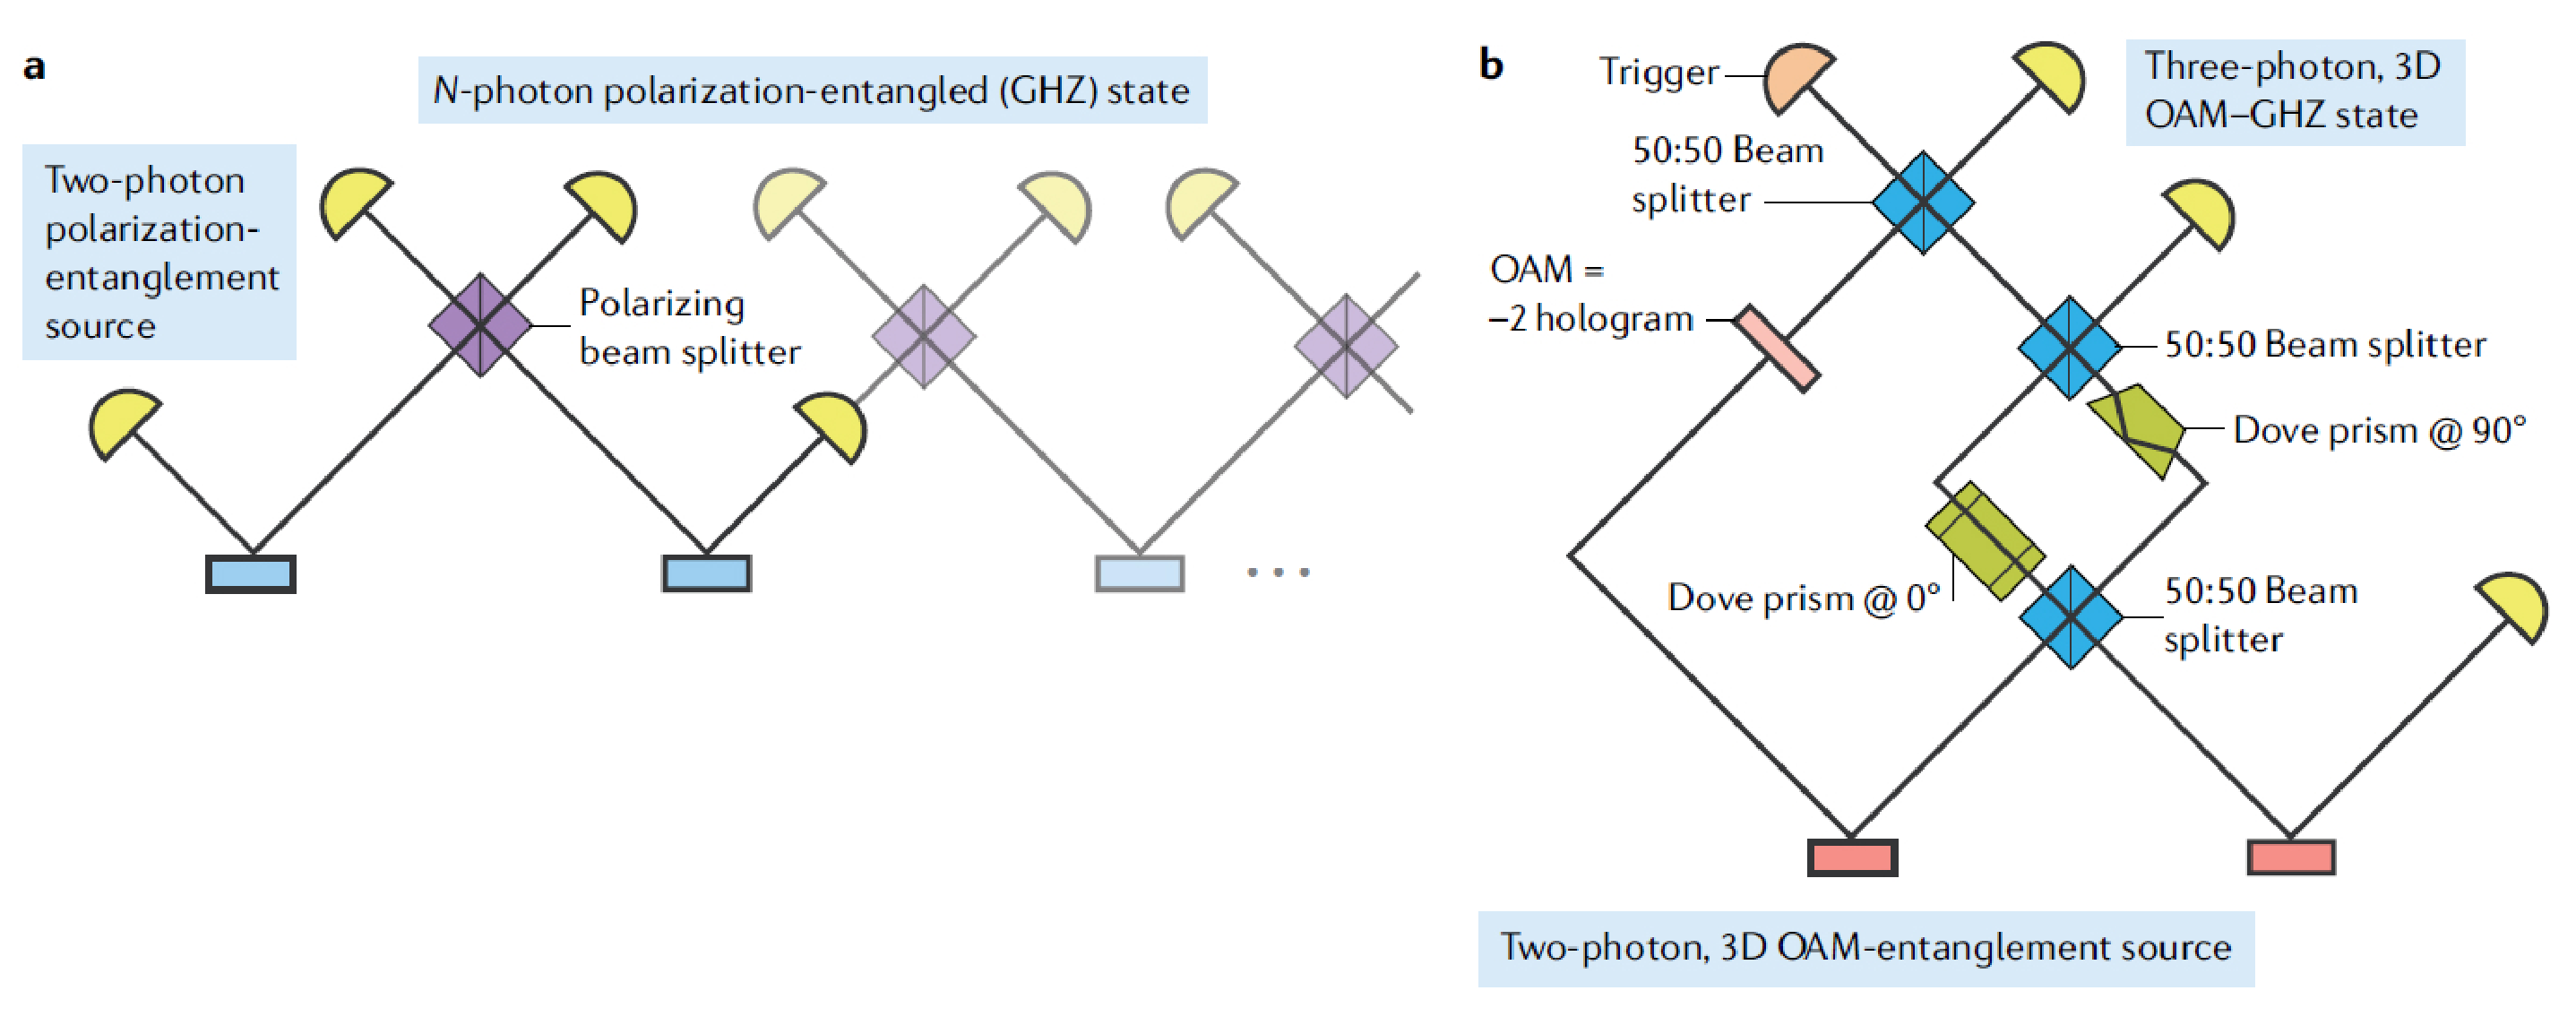
\includegraphics[width=\linewidth]{fig}
% \caption{\textbf{Title.} a | Text. b | Text. c | Text. d | Text maximum 250 words. Panel a is adapted/reproduced with permission from ref.123, Springer Nature Limited. Panel b is adapted/reproduced with permission from ref.124, Publisher Name.}
% \label{fig}
% \end{figure}



% \begin{table}[ht]
% \centering
% \begin{tabular}{|l|l|l|}
% \hline
% Particle & Mass & Charge \\
% \hline
 % \multicolumn{3}{|c|}{Charged particles}\\
% \hline
% Electron & $9.10938356(11)\times10^{-31}$ kg & $-1e$ \\
% \hline
% Proton & $1.672621898(21)\times10^{-27}$ kg & $+1e$ \\
% \hline
 % \multicolumn{3}{|c|}{Neutral particles}\\
% \hline
% Neutron & $1.674927471(21)\times10^{-27}$ kg & $0$ \\
% \hline
% \end{tabular}
% \caption{\label{tab}Tables have titles but no captions are allowed. All symbols and acronyms used in a table should be defined in a footnote. Example: Here $e$ is the elementary charge.}
% \end{table}


% \noindent\textbf{Acknowledgements}\\
% E.g. Funding agencies.\\

% \noindent\textbf{Author contributions}\\
% Please describe the contributions made by each author.  Please use the initials of the individual author to explain these contributions.  These contributions are also required when you upload the files to our submission website.\\

% \noindent\textbf{Competing interests}\\
% Nature Journals require authors to declare any competing interests in relation to the work described. Information on this policy is available \href{http://www.nature.com/authors/policies/competing.html}{here}. \\



% \noindent\textbf{Supplementary information (optional)}
% If your article requires supplementary information, please include these files for peer-review. Please note that supplementary information will not be edited.


\end{document}